\section{Complexity in Languages\timeestimation{30h}}
\label{sec:complexity}
While most languages we encounter are turing-complete, that does not need
to be the case. In this chapter, we will discuss the notion of a problem 
description as a programming language.

\subsubsection{Problem descriptions}
There are many different kinds of problems in computer science, for example 
sorting a list or determining if a boolean formula with variables is always
true. Nevertheless, these kind of problems are never singular -- we would not 
want an algorithm\footnote{Most definitions would not even allow this as an 
algorithm}, that could reliably sort the list $4, 8, 2, -9$, but one that 
could sort \emph{all} lists, no matter the size. This means of course, that 
algorithms need data as input to describe the problems they need to solve. 
This data is then called the \emph{problem description}. 

Looking back at the beginning, the semantic function was introduced to give 
meaning to data. Since then, we primarily used it to differentiate between 
\WHILE programs and the functions they denote. In the case of problem
descriptions, we can the interpretation of a problem would be the solution 
that we would expect. 

\begin{example}
	$U = Cons(Nil, Cons(Nil, Cons(Nil, Nil)))$, then $\interpret[unary]{U} = 3$.
\end{example}
\begin{example}
	$L=Cons(4, Cons(8, Cons(2, Cons(-9, Nil))))$ is the problem description for
	sorting the list $4, 8, 2, -9$ if given to a sorting procedure, formally
	$\interpret[sort]{L}= Cons(-9, Cons(2, Cons(4, Cons(8, Nil))))$. When given
	to a procedure, that calculates the minimum, the interpretation would be that
	instead, so $\interpret[min]{L} = -9$.
\end{example}

In this light, a problem description becomes a small and domain specific 
programming language, with the algorithm that solves it being an interpreter.
\subsection{Reductions}
Often in courses on algorithms, the same algorithm can be used in many 
different domains, because it has been observed that the two problems are 
\emph{essentially the same} or that one is \emph{essentially a special case of
another}. 

For example in chapter~\ref{Rice}, we saw that we could formulate any 
non-trivial function property as a halting problem. \TODO\lineofthought{Find good example}

\begin{defn}
	For a complexity class $X$, a $X$-\emph{reduction} of a problem $A$ to a
	problem $B$ is a compiler from the problem descriptions of $A$ to the 
	descriptions of $B$, so that compiling a description of $A$ and executing 
	it as a $B$ problem description is in $X$.
\end{defn}

\begin{example}
	The most common reductions are:
	\begin{enumerate}
		\item $\PTIME$-reductions translate and execute a problem in polynomial 
			time and therefore $\PTIME$ and $\PSPACE$ are closed under these reductions.
		\item Linear time reductions give much stronger bounds, so that for example
			a $O(n^2)$ problem to which another is reduced, proves that the other 
			problem is $O(n^2)$ as well.
		\item Computable reductions are used to show the computability or 
			incomputability of problems.
	\end{enumerate}
\end{example}

\subsection{Examples}
\subsubsection{Problems}
\paragraph{Factorization of binary numbers}
Given an integer $N$ to be factored and an upper bound $1<M<N$, is there a 
$1<d\leq M$ so that $\exists x\in \N: N = d\,x$. Or put in another way: is 
there a non-trivial divisor for $N$, that is no bigger than $M$.

It is obvious that the problem is contained in \NPTIME by the guess-and-check 
method. At first it might seem, that it is actually linear time: Just check 
up to $M$ if the counter divides $N$, but since $M$ is written in binary, it 
only takes $\log_2(M)$ space for the input, therefore counting up to the 
number is actually exponential in the input.
\begin{example}[Relevance] 
	The RSA algorithm for
	public key encryption allows to deduce the private
	keys from the public keys -- but only, if the
	attacker can factorize a big integer.
\end{example}

\paragraph{Context Free Grammar membership (CFG)}
A context-free grammar is a set of rules, how non-terminal symbols can be replaced by 
a mixture of again non-terminal symbols or terminal symbols (which can not be 
changed afterwards).

An easy example is the language of balanced braces:

\begin{grammar}
	<word> ::= <empty>
						\alt `(' <word> `)' <word>
						\alt `[' <word> `]' <word>
						\alt `{' <word> `}' <word>
\end{grammar}
which contains words like \texttt{([()()]\{\})} but not \texttt{(()}.

The problem is now, given a set of rules $R$, a start-token $A$ and a string 
$s$, to check whether $s$ could be produced from $A$ under the rules $R$. 
Without loss of generality, we can assume that each step produces at least 
one non-terminal character\citationneeded.

This is surely in \NPTIME, because if we were given the steps that expand $A$ 
to $s$, we could check that they do indeed produce $s$. There are however 
serveral algorithms, that efficiently expand the currently possible 
interpretations and can find the solution in
$\mathcal{O}\left( \abs{s}^3\,\abs{R} \right)$ time\footnote{See 
	\cite{sipser2006introduction}} and therefore the problem is also in \PTIME.
\begin{example}[Relevance]
	The syntax of programming languages is often
	described as a context free grammar (for example
	the syntax of \FOR in table~\ref{tab:FOR-syntax}).
\end{example}

\paragraph{Traveling Salesman Problem (TSP)}
A salesperson wants to travel to a number of locations across the country, 
but is interested in getting home as soon as possible. Given a map with 
travel times between the cities, is it possible to do the trip in time for 
their wedding anniversary in $k$ days?

More abstractly: Given a graph with weighted edges, is it possible to find a 
path crossing all nodes, so that the sum of the weights of the edges crossed 
is no bigger than $k$?
\begin{center}
	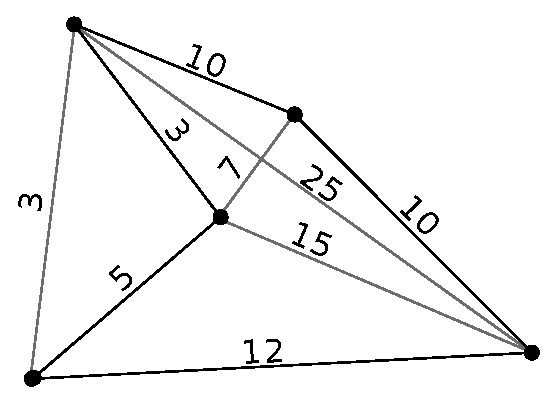
\includegraphics[height=3cm]{complexity/langcomplexity/pictures/tsp}
\end{center}
\begin{example}[Relevance]
	A circuit is basically a round-trip over a board. As such, minimizing 
	the resistance, \dots encompasses solving the TSP.
\end{example}

\paragraph{Satisfiability of boolean expressions (SAT)}
Given a boolean expression with variables, is there a way to assign the 
variables, so that the whole expression is true?
\begin{example}[Relevance]
	When modelling certain domains, for example in a system of artificial
	intelligence, constraints are often expressed as boolean expressions or can
	be converted to them\footnote{See \cite{russell1995artificial}}. Checking
	whether the constraints can be satisfied at all can already solve problems:
	If we have the facts $F$ and the hypothesis $H$, then $H$ fits the facts, if
	and only if $F\wedge\lnot H$ is \emph{not} satisfiable.
\end{example}
\subsubsection{Reductions}
SAT is an extremely handy problem to reduce to, so the following reductions 
will mostly feature that.
\paragraph{SAT reduces to TSP}
\TODO
\paragraph{TSP reduces to SAT}
\TODO
\paragraph{Factorization reduces to TSP}
\TODO

\paragraph{CFG reduces to SAT}
\TODO

\subsection{Hardness and completeness}
We saw that in computability, there seems to be a natural border of 
computability, in which \WHILE, Turing machines and nearly any reasonably 
strong language reside. It was not too surprising then, that these different 
languages could express each other and themselves by means of interpretation and
compilation. Maybe more surprising is, that the complexity classes \PTIME and 
\NPTIME seem to be a similarly natural border.

\begin{defn}
	For a complexity class $C$, a problem $P$ is \emph{hard}, if 
	$\forall c\in C: c \reducesTo P$.

	The problem $P$ is \emph{$C$-complete}, if $P$ is $C$-hard and $P\in C$.
\end{defn}
\begin{example}
	\begin{itemize}
		\item \FOR is \PTIME-hard, but not complete, because not all \FOR programms run in \PTIME.
		\item \TM is \WHILE-complete.
	\end{itemize}
\end{example}
These examples are a bit cheated, since they use extremely large complexity 
classes. But in fact, we have seen two problems already, that are \NPTIME-complete.

\subsubsection{SAT is \NPTIME-complete}
\begin{theorem}
	The satisfiability of boolean formulas is \NPTIME-complete.
\end{theorem}
\begin{proof}
	For completeness, inclusion and universality are required.

	To prove $SAT\in \NPTIME$, we use the guess-and-check definition of 
	\NPTIME. The required certificate in this case is a mapping of the variables to 
	truth-values. This is at most linear in the length of the expression, 
	therefore fulfilling the required \PSPACE length of the certificate. Given the 
	certificate, we can then fully evaluate the expression, which again takes 
	linear time.

	The general idea how to create an $X$-complete problem is to simulate the 
	mode of computation. In the case of space completeness, you fail if you 
	move out of a premarked part of the tape, in the case of 
	\PTIME-completeness, you count down your remaining time and in the case of 
	\NPTIME-completeness, you build a table of possible configurations of the 
	turing machine and see if any of them succeeds\footnote{This proof follows 
	\cite{sipser2006introduction}}.

	% Jones has a more elegant approach, but that requires to introduce the 
	% language SBoole, which then simulates a GOTO program, which simulates a 
	% TM. However the solution is so much prettier, that I consider adapting it 
	% to the known formalisms.
  %
	First assume without loss of generality, that the problem, we want to reduce
	takes at most $n^k$ steps to accept. This means, that we can be in at most 
	\TODO prove rest
\end{proof}
This implies, that SAT can express any other \NPTIME problem with only a 
polynomial slowdown. This also means, that SAT could model any \PTIME 
problem, such as checking context free grammar membership.

On the other hand, we saw that SAT can be reduced to the Traveling Salesman 
Problem, which shows its completeness as well.

There are indeed many relevant problems that are \NPTIME-complete\footnote{So 
many in fact, that the author struggled to find any interesting \PTIME problems}, for 
example maximizing linear functions over linear constraints in the domain of 
integers or optimal scheduling of tasks over multiple processors just to name two.

\subsubsection{\NPTIME and optimization}
\label{np-opti}
While one should keep in mind, that \NPTIME only
describes decision problems, many \NPTIME-complete
problems actually hide an optimization problem. For
example, if we can determine if the traveling
salesman can do the round-trip with cost of at most
$k$, then we can actually find the optimal path:

\begin{algorithmic}[1]
	\State find least $k_0$, so that the round-trip is possible with binary search over $k$
	\For{each edge $e$ in the graph}
		\State Remove the $e$
		\State Check if the round-trip cost increases
		\State If so, reinsert $e$
	\EndFor
\end{algorithmic}

After the algorithm finishes, the only edges in the graph are the ones in the round-trip.

\subsubsection{Help, my problem is \NPTIME-complete}
While being (probably) asymptotically very difficult to solve, 
\NPTIME-complete problems are by no means impossible. There are some 
strategies that can be applied to handle them.
\paragraph{\NPTIME-complete does not necessarily mean slow}
In many cases, the precise algorithm to solve the problem works reasonably 
fast in most cases, but explodes for some abnormal cases. If these abnormal 
cases don't occur in normal input data, the algorithm is still save.

For example, if we are solving SAT, but the inputs take only the form of horn 
clauses (for example $\bigwedge x_i \rightarrow y$), then the problem is 
solvable in \PTIME. 

It could also be, that the algorithm runs in $\mathcal{O}((1+\varepsilon)^n)$ 
for some small $\varepsilon$. Then $n$ would have to be very big for it to be problematic.
\paragraph{Parametrization}
The problem might be slow in general, but there are different parameters to 
the problem, that, when fixed, make the algorithm polynomial. Only increasing 
these parameters then give the full problem. 

For example, checking if a given program in the ML language\footnote{Java or
	C++ would be no better as anyone who ever used template code knows. Actually,
	C++ templates are even Turing-complete \cite{veldhuizen2003c++}}
does not violate any typing (i.e.\ a cast would be necessary) is
\NPTIME-complete\footnote{See \cite{downey1999parameterized}}, but if we
parametrize by the number of type definitions in the system, we have merely a
polynomial runtime.
\paragraph{Approximation}
As seen in section~\ref{np-opti}, many \NPTIME-complete problems are actually
optimization problems in disguise. Instead of looking for \emph{the} optimal
solution, often it is enough to settle for a sub-optimal, but good enough
solution.  In this text, we didn't develop the necessary tools to analyse such
inaccurate algorithms, but such algorithms can come --provably-- very close to
an optimal solution, while taking only polynomial time.

\subsection{Other complexity classes}
The complexity classes introduced are of course only scratching the surface 
of the fascinating topic of complexity theory. There are many different modes 
of computation, that do not factor into \PTIME or \NPTIME, for example 
parallelism, which will be of ever greater importance, as the number of cores 
of computers increase, when the sequencial speed cannot. A bit further down 
the road, the quantum computer will get its share.

\paragraph{$\mathtt{NC}$}
stands for Nick's class\footnote{honoring Nick Pippenger} and
has been described as the class of well-parallelizable 
problems\citationneeded. It is known that $\mathtt{NC} \subset \PTIME$, but it is unknown, 
whether this inclusion is proper. Similarly to \NPTIME-complete problems, 
\PTIME-complete problems, such as CFG, are analyzed to prove this. 

\paragraph{$\mathtt{BQP}$}
is the class of bounded-error polynomial-time quantum computable decision 
problems. Bounded error compensates for the fact that quantum computation is, 
in order to achieve its full strength, random. Bounding the error means that 
it gives the wrong answer at most $0<\varepsilon<\frac{1}{2}$ of the time, where 
$\varepsilon$ is often arbitrarily chosen to be $\frac{1}{3}$. Given a 
procedure in $\mathtt{BQP}$, it is easy to see, that we can lower the 
probability of error arbitrarily low by running the procedure multiple times 
and taking the average answer.

It is possible to simulate a quantum computation in \PSPACE, and it is 
possible to simulate a deterministic computation on a quantum computer, so 
$\PTIME \subset \mathtt{BQP} \subset \PSPACE$, but again, all inclusions are 
suspected, but not proven, to be proper.

The connection to \NPTIME is unknown, but $\NPTIME\subset \mathtt{BQP}$ would 
imply $\NPTIME\neq \PTIME$.

\subsection{Why \PTIME is probably not \NPTIME}
\cite{impagliazzo1995personal}
